\documentclass[12pt]{article}

\usepackage{graphicx}
\usepackage{amsmath}

\title{An approach to breast tumor classification using an active learning method}


\author{Shaan Varia \\ Carnegie Mellon University \and Akul Penugonda \\ Carnegie Mellon University}

\begin{document}

\maketitle

\section{Introduction}

Currently, the scenario in an oncologists room is thus: a patient enters with a potential tumor determined by a mammogram performed on the patient, which is diagnosed by a doctor as either possibly malignant or benign. If possibly malignant, a biopsy is performed to verify. A biopsy can cost anywhere from \$150 to \$10000, and is a painfully invasive procedure which should be avoided if possible, for both cost and comfort. An active learning approach could result in a lot of saved money and pain for the patient. In this paper, we discuss an application of DHM to a mammographic mass dataset, using only features which may be acquired by non-invasive methods, namely a mammogram.  Our results show that DHM's learning approaches the accuracy of a supervised learner, indicating potential benefits to using this method in the real world.

\section{Background}

A mammogram yields three features that are characteristic of tumors when there is a mass in the breast. These three features are shape of mass in the breast, margin of the mass, and density of the mass. We will use these together with the age of the patient to predict severity, i.e. whether the mass in the patients breast is benign or malignant. Before discussing the learner, we will go over the role that each of these features play in relation to the mass observed being malignant or benign.

\subsection{Density}

Density of mammographic mass does not refer to the traditional definition of density (mass/volume), rather it refers to the amount of fat and tissue in the breast. A dense breast is one that has more tissue than fat. Studies have shown that women with high breast density are 4-5 times more likely to develop breast cancer compared to women with low breast density \cite{boyd, white}. 

Density is an ordinal field - that is, the higher the density the higher the chance of the mass being malignant.

\subsection{Margin}

Margin refers to what the outer part of the mass looks like. Margin of the mammographic mass is a nominal field, and as such we will go into the distinctions between the classes. 

\subsubsection{Circumscribed}

The mass is surrounded by tissue and is not as likely to be malignant, most circumscribed margins are likely to be benign \cite{shapeMarginDensity, birads}.

\subsubsection{Microlobulated}

Microlobulated breast margins refer to many small lobulations on the surface of a breast nodule. If more of these microlobulations pop up on the mass then there is a higher chance of the mass being malignant \cite{benignOrMalignant}, and as such microlobulated masses are treated with more care, and are not simply passed off as benign.

\subsubsection{Obscured}

Obscured breast margins are suspicious due to the fact that they cannot be discerned.

\subsubsection{Ill-defined/Irregular}
An ill defined margin is one that cannot be distinguished from the fatty tissue surrounding it. This may mean that the mass is invading the tissue, which would be an indicator of malignancy.

\subsection{Shape}

Shape is similarly a nominal field, and simply refers to the visual shape of the mass as observed on the mammogram \cite{barnes}.
\subsubsection{Round, Oval, Lobular}
All of these shapes are not highly indicative of malignancy. Lobular masses refer to those who have small undulations on the mammogram.
\subsubsection{Irregular}
Irregular masses are indicative of malignancy by virtue of the fact that they are not the regular shapes of common benign masses such as fibroadenomas or cysts.

\subsection{Related Work}

There is a large corpus of papers using machine learning to predict the incidence of disease. Shipp and Ross (2002) created a supervised learner to predict lymphoma outcomes for two classes of patients \cite{shipp}. SVMs have also been used in the classification of leukemia, colon cancer, and ovarian cancer. The hardest part about this classification is the high dimensionality of microarray results in relation to the number of samples actually available \cite{review}.

Zhang used a similar mammographic mass set to create a neural-genetic algorithm that performs binary classification. This method obtained an 87.2\% success rate \cite{zhang} Elter et al. proposed two different learning methods on this data set. The first method was a decision tree. The second method relies on case-based reasoning. Both of these methods outperform an artificial neural network, and both also use the BI-RAD feature. \cite{predictionCAD}. 

Our project differs from these in that we do not use the BI-RAD feature of the data, and we similarly are taking an approach that relies on only the results of a mammogram.

\section{Methods}

\subsection{Data Source}

We got our data from the UCI machine learning repository. The below data set has 961 entries, where each entry contains the following features and labelings: 

6 Attributes in total (1 goal field, 1 non-predictive, 4 predictive attributes) 
\begin{enumerate}
\item BI-RADS assessment: 1 to 5 (ordinal, non-predictive!) 
\item Age: patient's age in years (integer) 
\item Shape: mass shape: round=1 oval=2 lobular=3 irregular=4 (nominal) 
\item Margin: mass margin: circumscribed=1 microlobulated=2 obscured=3 ill-defined=4 spiculated=5 (nominal) 
\item Density: mass density high=1 iso=2 low=3 fat-containing=4 (ordinal) 
\item Severity: benign=0 or malignant=1 (binominal, goal field!) 
\end{enumerate}

Taken from \cite{dataset}.

We did not use BI-RADS as it is too predictive of a feature. We will instead just use Age, Shape, Margin and Density to predict Severity. The above data set contains 516 benign entries and 445 malignant entries and as such is fairly evenly distributed.

\subsection{Active Learning}
As discussed in the introduction we envision the following scenario. We are running a hospital which offers mammograms and biopsies to patients and we need some metric to determine which patients need to go for a biopsy after having a mammogram taken. We will not use BI-RADS at all to make this decision as BI-RADS is simply an aggregative result based on the information gleaned from the mammogram. As in any hospital setting we cannot choose which patients we receive and at what times. Thus we are led to adopt a streaming data model for our active learning algorithm. Similarly, we only get one shot to run our algorithm as there are no do overs in the medical world and we are not able to change our algorithm whilst it is making predictions for patients. This leads us to fix a random seed to our data and ensure that a specific ordering takes place (such that each run isn't reliant on the whims of the random number generator).

We applied DHM to a fixed random subset of 100 data points from the total set. This was meant to simulate the stream of patients that a hospital receives. In the DHM algorithm there are 4 major areas that need to be discussed, namely: using SVM's to represent our hypotheses, the calculation of errors on our positive and negative hypotheses, the generalization bound Delta, and the consistency of hypotheses from iteration to iteration.

\subsubsection{Support Vector Machines}
Our algorithm utilized Matlab's built in Support Vector Machine framework to represent our hypotheses. This allows us to facilitate binary classification in an easy manner. We used the standard linear kernel built in to Matlab, and as we will see later, this makes calculation of delta easy.

\subsubsection{Calculation of Error on Hypothesis}
We calculate $err(h_{+1/-1},S\cup T)$ by using the respective positive and negative hypotheses to predict all the labels for the points in $S\cup T$. We then compare these predicted labels to what our algorithm has previously predicted the labels as, and return the proportion of labels that don't agree.

\subsubsection{Generalization Bound Delta}
As per Dasgupta and Hsu's implementation of DHM, a generalization bound Delta need be calculated. This generalization bound is of the following form:

\begin{align*}
\Delta_t &= \beta_t^2+\beta_t(\sqrt{err(h_{+1},S\cup T)}+\sqrt{err(h_{-1}, S\cup T)})\\
\beta_t&= C\sqrt{\frac{d \log t + \log(1/\delta)}{t}}
\end{align*}

where $d$ is the VC dimension of our hypothesis, $C$ is a universal constant and $\delta$ is the overall permissible failure probability \cite{DH}. Due to the fact that our hypotheses are Support Vector Machines with a linear kernel our VC dimension is simply the number of features we have plus one. Thus, in this case our VC dimension is 5. We have chosen $\delta$ as 5\%. 

\subsubsection{Consistency of Hypotheses}
An important part of DHM is measurement of the consistency of hypotheses when learning $h_{+1}$ and $h_{-1}$. We tried multiple different methods of comparing consistency including counting the number of support vectors in the old and new hypotheses and measuring their difference, as well as attempts at using statistical t-tests and thresholding. However, we found that these did not work as well and instead said that a hypothesis was consistent if its error is no larger than the previous hypothesis' error (using $err(h_{+1/-1/old}, S\cup T)$).

\subsection{Supervised Learning}

We have also included a supervised learner which learns alongside the active learner but on every iteration of the algorithm asks the oracle for a label for the given point. We can imagine the supervised learner as a doctor who wants to completely remove all possibility of false negatives, and as such sends every patient that comes in for a biopsy. Whilst this is an obscure notion, one could foresee a clinic in which a similar case was happening. 

\section{Results}
Our active learning strategy achieves a 21.75\% generalization error rate. Looking at figure \ref{fig:generr}, we see that our active learner converges to the same error rate that our supervised learner achieves. What is interesting is that unlike the supervised learner, we only query from the oracle 44 times (as seen in figure \ref{fig:costcurve}) which is less than 50\% of the number of times the supervised learner queries.

We achieve a precision of 72.69\%, recall of 84.94\% and as such our final F1 score is 78.34\%, as seen in \ref{fig:precisionrecall}.

\begin{figure}
	\centering
	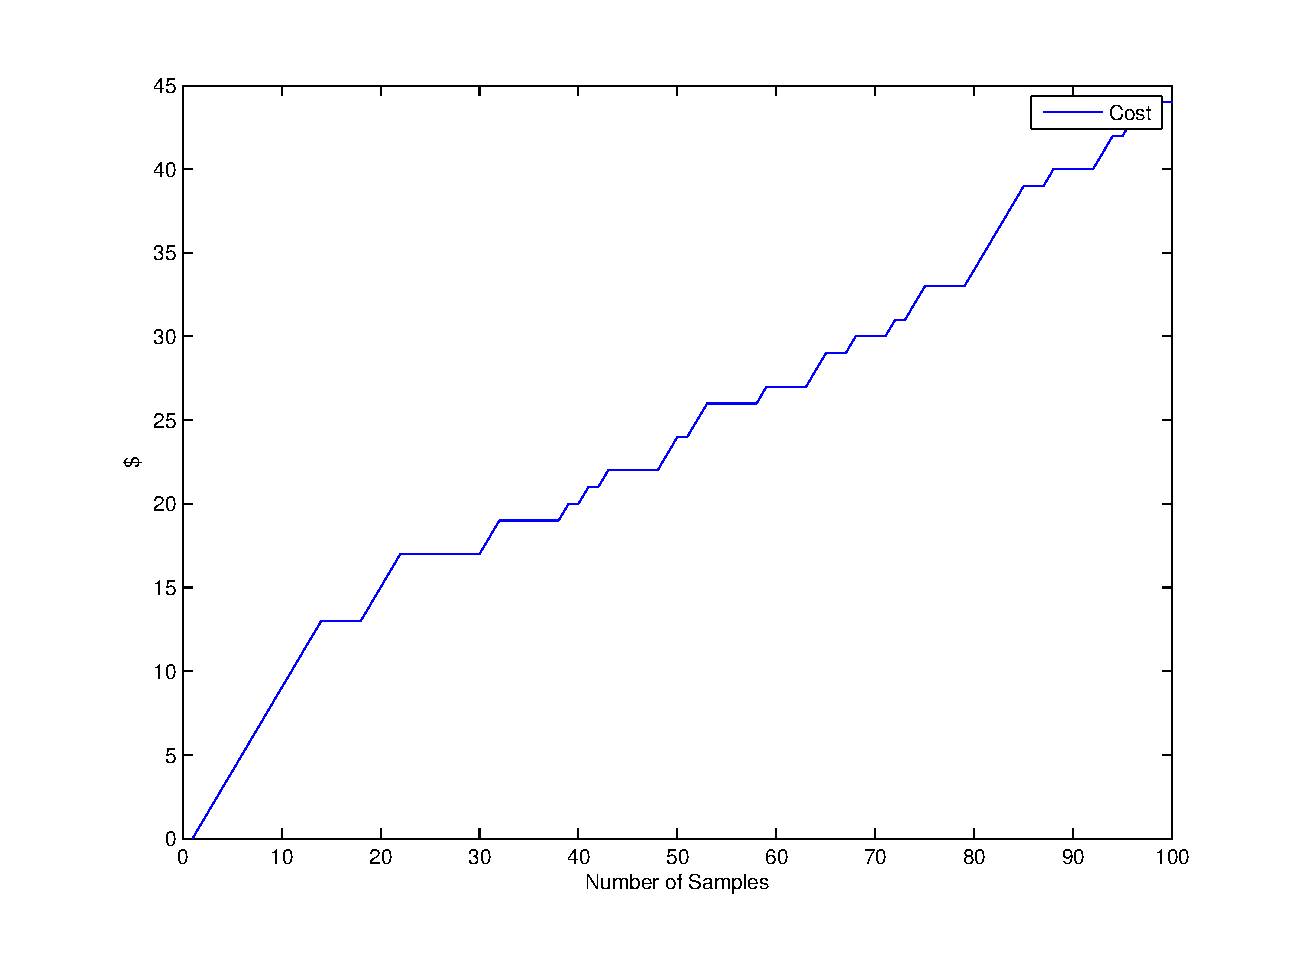
\includegraphics[width=300px]{costcurve}
	\caption{Cost Curve}
	\label{fig:costcurve}
\end{figure}

\begin{figure}
	\centering
	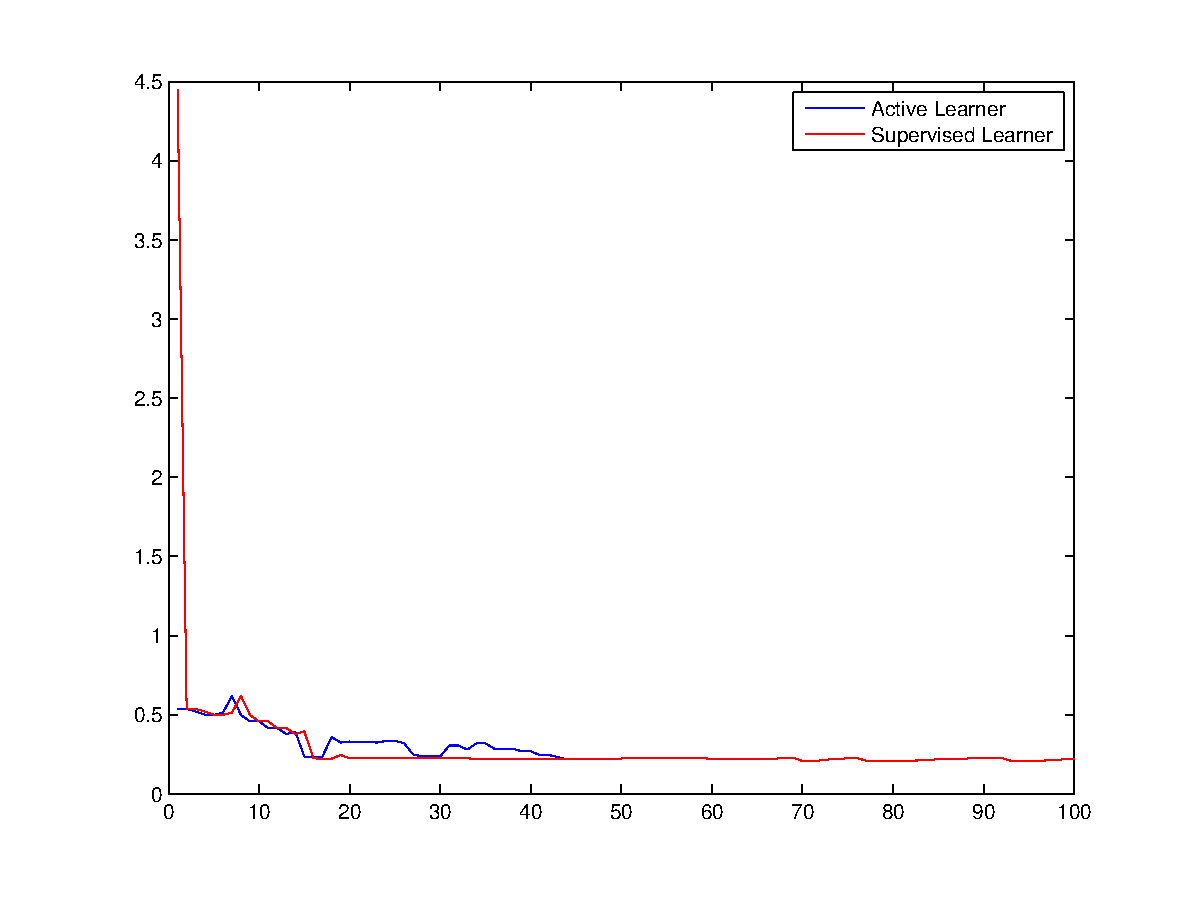
\includegraphics[width=300px]{generr}
	\caption{Generalized Error}
	\label{fig:generr}
\end{figure}

\begin{figure}
	\centering
	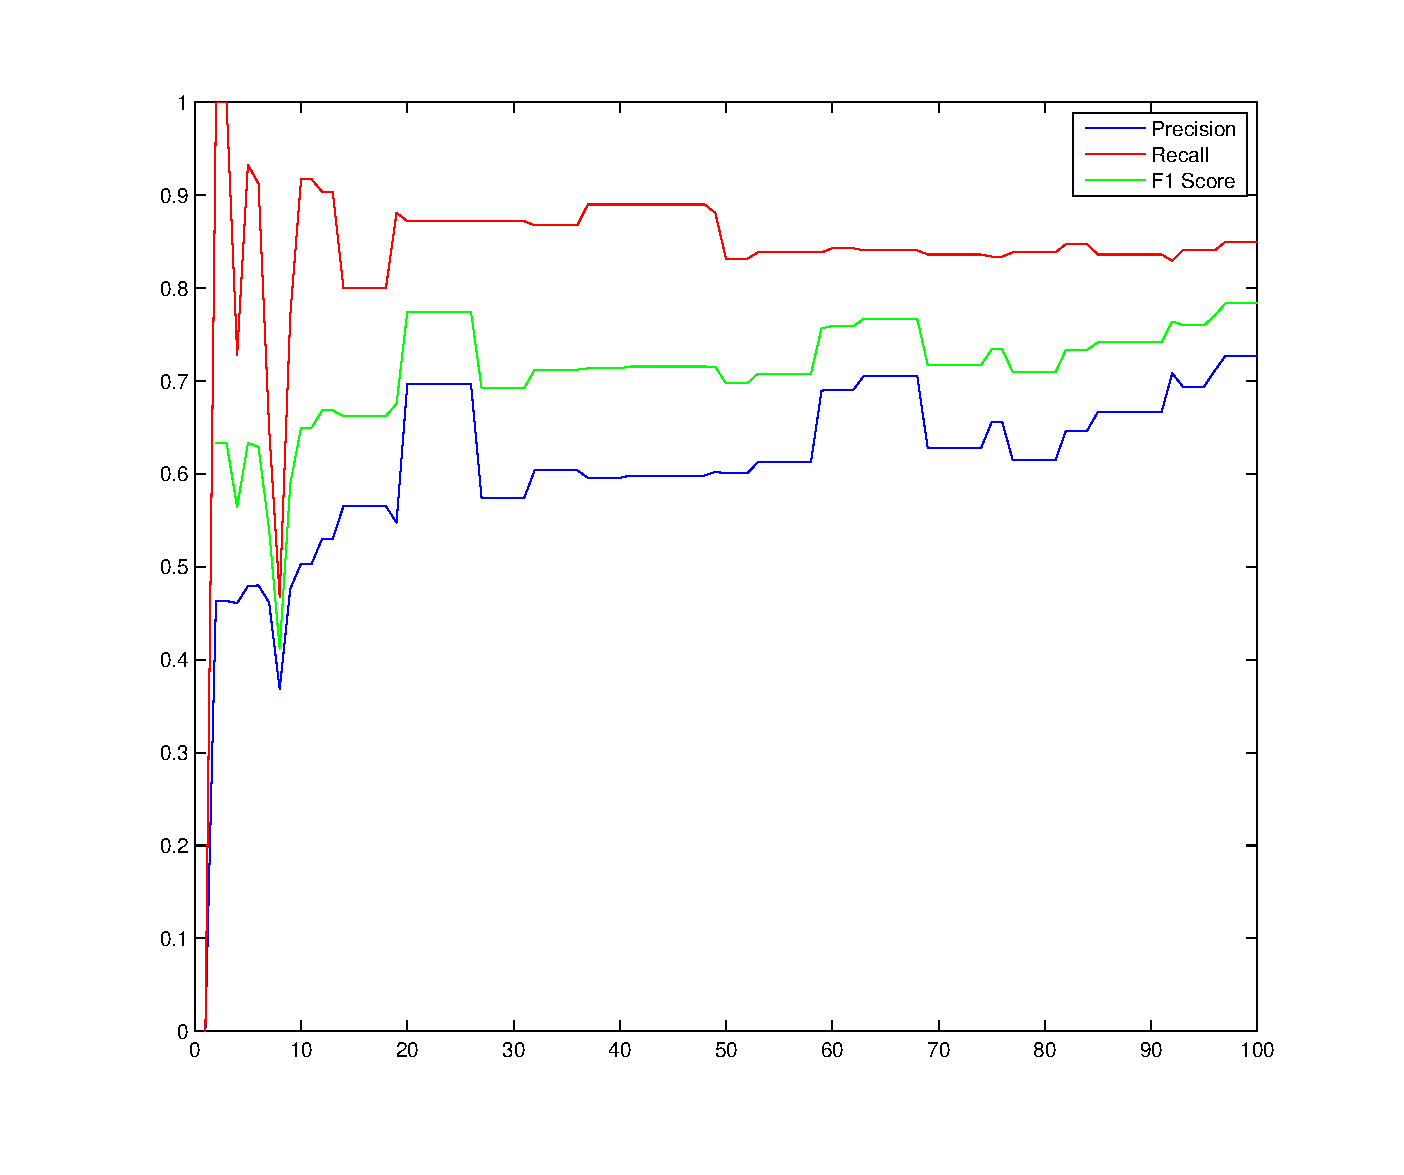
\includegraphics[width=300px]{precisionrecall}
	\caption{Precision, Recall, and F1 Score - Active Learner}
	\label{fig:precisionrecall}
\end{figure}

\begin{figure}
	\centering
	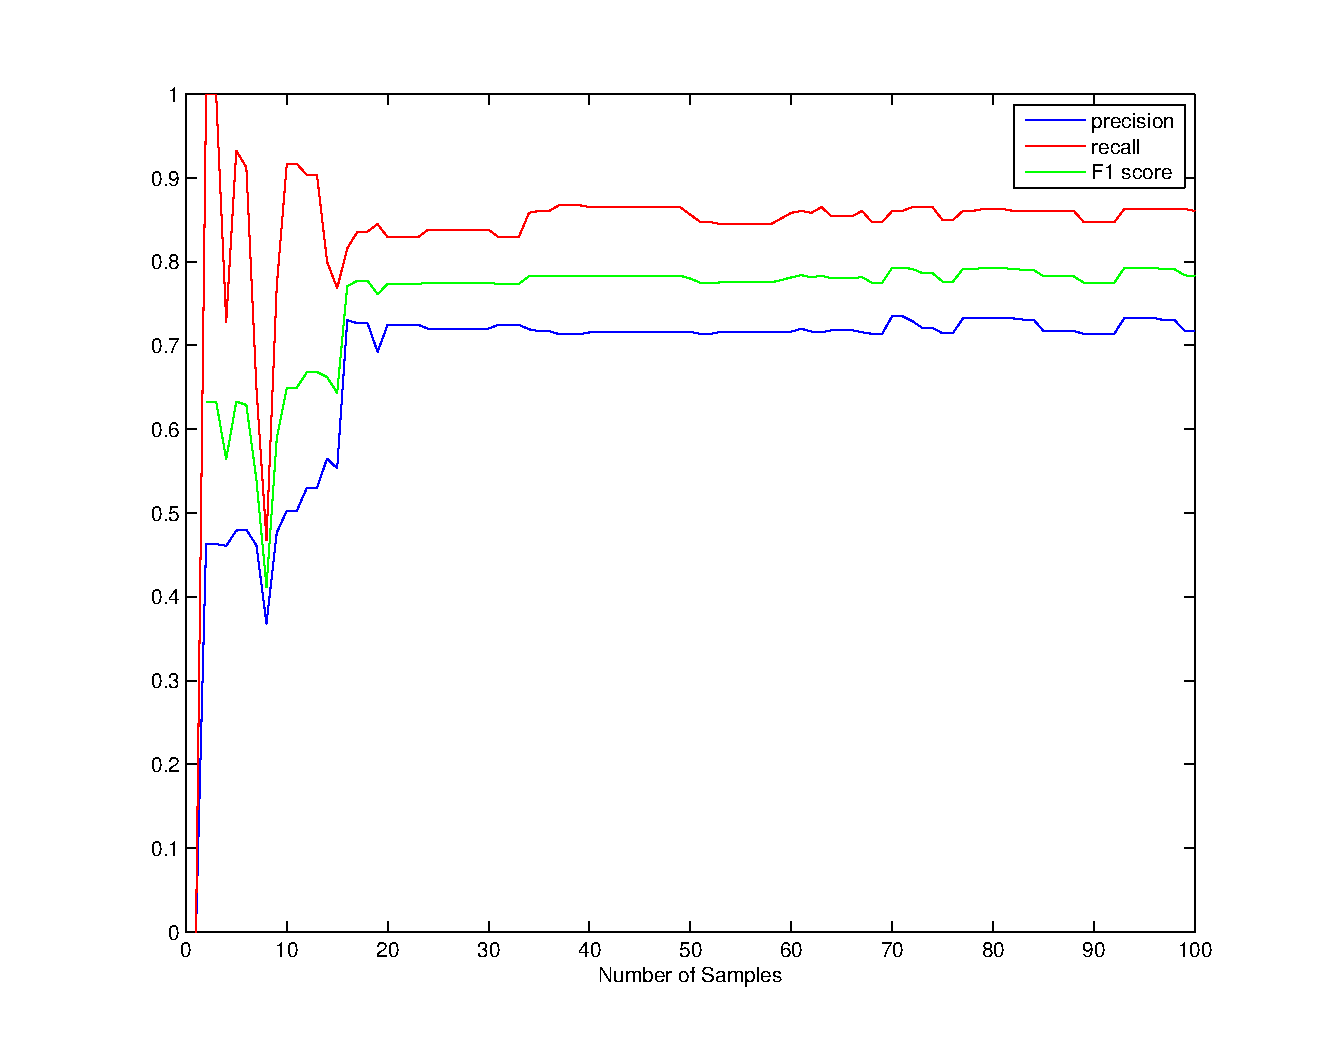
\includegraphics[width=300px]{precisionrecallSup}
	\caption{Precision, Recall, and F1 Score - Supervised Learner}
	\label{fig:precisionrecallSup}
\end{figure}



\section{Discussion}
As seen in Figure \ref{fig:generr} we converge in error rate to a supervised learner which queries the oracle on every new point. We only query the oracle a total of 44 times (as seen in Figure \ref{fig:costcurve}) which is less than half of the initial stream of 100 data points seen. This means that our method is inferring more than half of the points with the same error rate as the supervised learner. The cost savings of this are huge especially when factoring in the cost of a biopsy. This is due to the fact that we only go to the oracle for points that are close to the margin (i.e. points that are consistent under both the positive and negative hypothesis). This approach to inference works incredibly well with support vector machines which try and maximize the distance from points to the margin of separation, as it becomes very clear which points are near the margin.

We notice that our cost curve (Figure \ref{fig:costcurve}) increases linearly initially and then has patches in which no queries to the oracle are performed. This makes sense as the initial points give a lot of information to the support vector machine, and allow it to stratify its margin. Once it has acquired a sufficient number of points, inferences can start to be made. We observe that this point of 'sufficiency' occurs at around 15 queries to the oracle.

From Figure \ref{fig:precisionrecall}, we can see that the precision, recall, and F1 score for our active learner all peak early on. This is likely due to chance - the learner simply picks a couple points that happen to be very representative of the model as a whole. The collective dip around the 10pt mark indicates the curve overcorrecting as it receives more data. Precision, recall and F1 score all continually increase as more samples are received - this indicates that the model is becoming more and more accurate.

We can see that the supervised learner's curves are much different in Figure \ref{fig:precisionrecallSup}. It too peaks early on, then dips and recovers. However when it comes back up, it comes back up to a plateau. This indicates that though it receives more samples, it is not getting better. The active learner, though, continuously gets better until it also hits a plateau, at about the same level as the supervised learner. This shows that the active learner approaches the performance of the supervised learner, even while using less samples.

\section{Conclusion}

It is clear that our DHM achieves near parity to a supervised learner, while using less than half of the samples. A doctor using this DHM approach could expect to spend less than half what they currently spend on biopsies (assuming that they currently make all of their suspect patients receive biopsies). DHM would be a supplemental aid for doctors who are diagnosing patients. 

\subsection{Future Work}
An important aspect of the diagnosis process is the role of false negatives, i.e. malignant tumors not sent to biopsy. Doctors usually err on the side of reducing false negatives to 0 as it is much less costly to have a patient go for a biopsy and not have cancer, than for them to not go for a biopsy but have cancer. Doctors take this into account when determining which patients to send for biopsy, however we have not considered this at all. A method to overcome this might involve giving the weighing our hypotheses in such a way that sends more people for biopsies if they are near the margin of our support vector machine. This would be a further area of study and might yield some interesting results.

We have a somewhat high false positive rate. We could expand our learner to use more features i.e. BI-RADS as a confirmatory measure. Also, we chose to represent our hypothesis as an SVM. It is possible that a k-d tree would be more useful for this sort of classification. More experimentation with different hypothesis models would be better to determine the best approach.

\bibliography{myBib}{}
\bibliographystyle{plain}
\end{document}